\documentclass{article}

\usepackage{latexsym, amsmath, amsfonts}
\usepackage{hyperref}
\usepackage{tikz}
\usetikzlibrary{arrows}

\title{Breadth-first search}
\author{Juan M. Barrios}

\begin{document}

  \maketitle

  \begin{abstract}
    In graph theory, breadth-first search (BFS) is a strategy for searching in a graph when search is limited to essentially two operations: (a) visit and inspect a node of a graph; (b) gain access to visit the nodes that neighbor the currently visited node. The BFS begins at a root node and inspects all the neighboring nodes. Then for each of those neighbor nodes in turn, it inspects their neighbor nodes which were unvisited, and so on. Compare BFS with the equivalent, but more memory-efficient Iterative deepening depth-first search and contrast with depth-first search.
  \end{abstract}

  \tableofcontents

\section{Algorithm}

  The algorithm uses a queue data structure to store intermediate results as it traverses the graph, as follows:
  \begin{enumerate}
    \item Enqueue the root node.
    \item Dequeue a node and examine it.
    \begin{itemize}
      \item If the element sought is found in this node, quit the search and return a result.
      \item Otherwise enqueue any successors (the direct child nodes) that have not yet been discovered.
    \end{itemize}
    \item If the queue is empty, every node on the graph has been examined – quit the search and return ``not found''.
    \item If the queue is not empty, repeat from Step 2.
  \end{enumerate}
  \textbf{Note:} Using a stack instead of a queue would turn this algorithm into a depth-first search.

  In Figure~\ref{F:bgs}, we can see the order in which nodes are expanded by the Breadth-first search.

  \begin{figure}
    \centering
      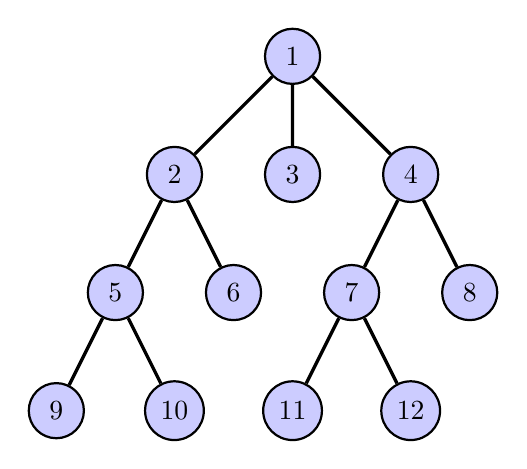
\begin{tikzpicture}[every node/.style={minimum size=7mm, circle, draw=black, fill=blue!20, thick}, very thick]
        \node {1}
          child{ node{2} 
            child{ node{5} 
              child{ node{9} }
              child{ node{10} }
            }
            child{ node{6} }
          }
          child{ node{3} }
          child{ node{4} 
            child{ node{7} 
              child{ node{11} }
              child{ node{12} }
            }
            child{ node{8} }
          };
      \end{tikzpicture}
    \caption{Order in which the nodes are expanded}\label{F:bgs}
  \end{figure}
  

  \subsection{Pseudocode}
  \textbf{Input:} $A$ graph $G$ and a root $v$ of $G$

  \begin{verbatim}
  1  procedure BFS(G,v) is
  2      create a queue Q
  3      create a set V
  4      enqueue v onto Q
  5      add v to V
  6      while Q is not empty loop
  7          t ← Q.dequeue()
  8          if t is what we are looking for then
  9              return t
  10         end if
  11         for all edges e in G.adjacentEdges(t) loop
  12             u ← G.adjacentVertex(t,e)
  13             if u is not in V then
  14                  add u to V
  15                  enqueue u onto Q
  16             end if
  17         end loop
  18     end loop
  19     return none
  20 end BFS
  \end{verbatim}

  \section{Features}

  \subsection{Space complexity}

  When the number of vertices in the graph is known ahead of time, and additional data structures are used to determine which vertices have already been added to the queue, the space complexity can be expressed as $O(|V|)$ where $|V|$ is the cardinality of the set of vertices. If the graph is represented by an Adjacency list it occupies $\Theta(|V|+|E|)$ space in memory, while an Adjacency matrix representation occupies $\Theta(|V|^2)$.

  \subsection{Time complexity}

  The time complexity can be expressed as $O(|V|+|E|)$ since every vertex and every edge will be explored in the worst case. Note: $O(|E|)$ may vary between $O(|V|)$ and  $O(|V|^2)$, depending on how sparse the input graph is (assuming that the graph is connected).

  \section{Applications}

  Breadth-first search can be used to solve many problems in graph theory, for example:
  \begin{itemize}
    \item Finding all nodes within one connected component
    \item Copying Collection, Cheney's algorithm
    \item Finding the shortest path between two nodes u and v (with path length measured by number of edges)
    \item Testing a graph for bipartiteness
    \item (Reverse) Cuthill–McKee mesh numbering
    \item Ford–Fulkerson method for computing the maximum flow in a flow network
    \item Serialization/Deserialization of a binary tree vs serialization in sorted order, allows the tree to be re-constructed in an efficient manner.
    \item Construction of the failure function of the Aho-Corasick pattern matcher.
  \end{itemize}

  \subsection{Finding connected components}

  The set of nodes reached by a BFS (breadth-first search) form the connected component containing the starting node.

  \subsection{Testing bipartiteness}

  BFS can be used to test bipartiteness, by starting the search at any vertex and giving alternating labels to the vertices visited during the search. That is, give label 0 to the starting vertex, 1 to all its neighbours, 0 to those neighbours' neighbours, and so on. If at any step a vertex has (visited) neighbours with the same label as itself, then the graph is not bipartite. If the search ends without such a situation occurring, then the graph is bipartite.
\end{document}